% A brief overview of Localisation is given in
% Section~\ref{sec:Localisation}, followed by an overview of SLAM in
% Section~\ref{sec:SLAM}. Finally the problem of cycle detection or
% ``loop closing'' is discussed in Section~\ref{sec:back_loop}.

\section{Lessons from Biology}

A lot of robotics research is biologically inspired. There are plenty
of primitive tiny creatures in the natural world capable of
very sophisticated behaviour. It is inspiring for a robotics
researcher to know that complex tasks can be achieved with very
limited resources, and we can learn how it can be done by studying
biological systems.

Of particular interest to this thesis are the navigational skills that
many organisms possess. It is generally assumed that sophisticated
navigational behaviour can only be made possible if an organism
maintains some form of map of the environment in their brain.  A good
overview of robotics research that mimics the navigational behaviour of
biological systems is given in \cite{bio_franz00}.

It is generally a difficult problem to decipher the exact
representation an animal is using to describe the environment. There
is only so much one can recover from observing the behaviour of an
animal. We will therefore concentrate on the studies of the spatial
representation in humans.

%{\bf Humans}\\ 
Early research in spatial representation in humans
\cite{psycho_piaget56} assumed that environmental representations are
actually stored in the brain in cartographic form.  Piaget believed
that a child's intellectual development can be divided into four
discrete stages. These are more than just convenient ways of breaking
down a description of child development. He believed that each stage
represents a qualitatively different type of understanding of the
world from the previous one, and not just a quantitative increase in
knowledge of the world. Piaget proposed the following stages:

\begin{enumerate}
\item Sensorimotor Intelligence\\
   The child's thought is almost entirely perceptual and is based on 
   interactions with objects in the environment. Representation of the
   environment is relative to his own body only.

\item Preoperational Intelligence\\
   The child's thought starts getting detached from the immediate
   environment. Objects and places in the external world become
   symbols in the mind, which can then be manipulated in a fairly
   limited way. Reasoning is intuitive rather than logical, and
   knowledge is relatively unstructured.

\item Concrete Operational Intelligence\\ 
    The child is able to imagine multiple perspectives on a situation.
    He realises that a sequence of actions can be cancelled out by
    the reverse sequence, and that the same goal can be achieved by a
    number of different means.

\item Formal Operational Intelligence\\
    Thinking becomes abstract and logical, free from direct experience.


\end{enumerate}

Piaget's theory of spatial development traces the evolution of
understanding of two related concepts: projective relations and
Euclidean geometry. As the child develops through successive stages of
cognitive structure, these concepts develop in parallel, but also
become increasingly coordinated. The child develops from early stages,
where spatial thinking is tied to his own experience and images of
the environment, to one where higher-order logical properties
(e.g. the formal mathematical and geometrical properties of a
Cartesian or Euclidean coordinate system) are applied to the relative
locations of objects in space.

The rough robotic analogy of these stages would be
\begin{enumerate}

\item No map at all, reactive navigation with collision avoidance,
  odometry-based localisation.

\item Set of routes - topological maps without cycles.

\item Topological maps with cycles.

\item Global map with single reference frame. Relative locations of
  all landmarks are known with some certainty.
\end{enumerate}

Similarly to Piaget, Siegel \& White \cite{psycho_siegel75} proposed
that adults construct a cognitive representation of the physical world
at two levels. At the first level, sequences of landmarks are linked
to the route. Each landmark has directional information attached to
it: ``turn left after passing 7/11 store''. Distances are left
unspecified. As an adult gains experience of the environment, he
incorporates a sense of relative distances between landmarks. As this
information gets incorporated into the map it becomes possible to
recover bearing between any two points in the environment regardless
of whether or not they are adjacent.

Siegel \& White \cite{psycho_siegel75} see this process as the first
step in the coordination of routes into a fully metric survey-like
representation of the environment (equivalent of stage 4 in Piaget model).

However, many researchers disagree with the idea that the human brain
stores a cartographic representation of the environment. Kuipers
\cite{psycho_kuipers82} argues that such a single metric
representation would commit the system to a high degree of accuracy
and would thus not support states of partial knowledge. He argues that
a single mistake on such a representation would be very costly to
rectify at a later date, requiring the readjustment of large portions
of the representation.

Golledge \cite{psycho_golledge87} suggested that we may accurately
represent the metric relations (i.e. distance and direction) between a
limited number of major reference points, and that these then become
fixed points of reference for more local groupings at a lower
hierarchical level. We thus locate one of the minor landmarks by first
orienting ourselves towards its nearest major reference landmark; from
this we can then infer the route to the minor landmark. The relative
orientations of the fixed systems are poorly specified and retain some
subjective component; thus it is problematic to infer relative
location directly between minor points in different systems. One must
rather go up and down in the hierarchy.

%%% I personally tend to agree more with Golledge's point of view. For
%%% instance I can easily point in the direction of the coffee machine
%%% when I am in my office at university, in addition, I can tell how it
%%% is oriented relative to my desk.  However I can provide only a rough
%%% estimate of the direction to my house, and a rather poor distance
%%% estimate, and I am really uncertain about the orientation of my house
%%% relative to the coffee machine in the university. 

%need a summary on the observation that local things are
%  metric, but further things are topological.

%Other interesting references: 
\nocite{psycho_tversky81}
\nocite{psycho_mcnamara86} 
\nocite{psycho_passini84}
\nocite{psycho_piaget60}

\section{Robotic Mapping}

%Introduce metric/topological mapping. Introduce EKF, FastSLAM, EM. State
%how topological and metric were rather disjoint. Maybe borrow some text
%from the next section. Future reference to the next chapter that defines
%EKF and FastSLAM in a formal way.

There are two main paradigms of robotic mapping: topological and
metric. The topological map is essentially a graph.  Nodes of the
graph represent places in the environment. Edges of the graph
correspond to routes between places. Every edge contains some
information on how to get from one node to another. This information
can be metric (e.g. go east for about 10m), but is generally too
coarse, sufficient only to get a robot moving in the right direction.
The robot is expected to rely on its path following (go down the
corridor, for example) and place recognition skills for navigation. An
example of a topological map used by people is a subway schematic (See
\refFigure{fig:subway}).

\begin{figure}[h]
\begin{center}
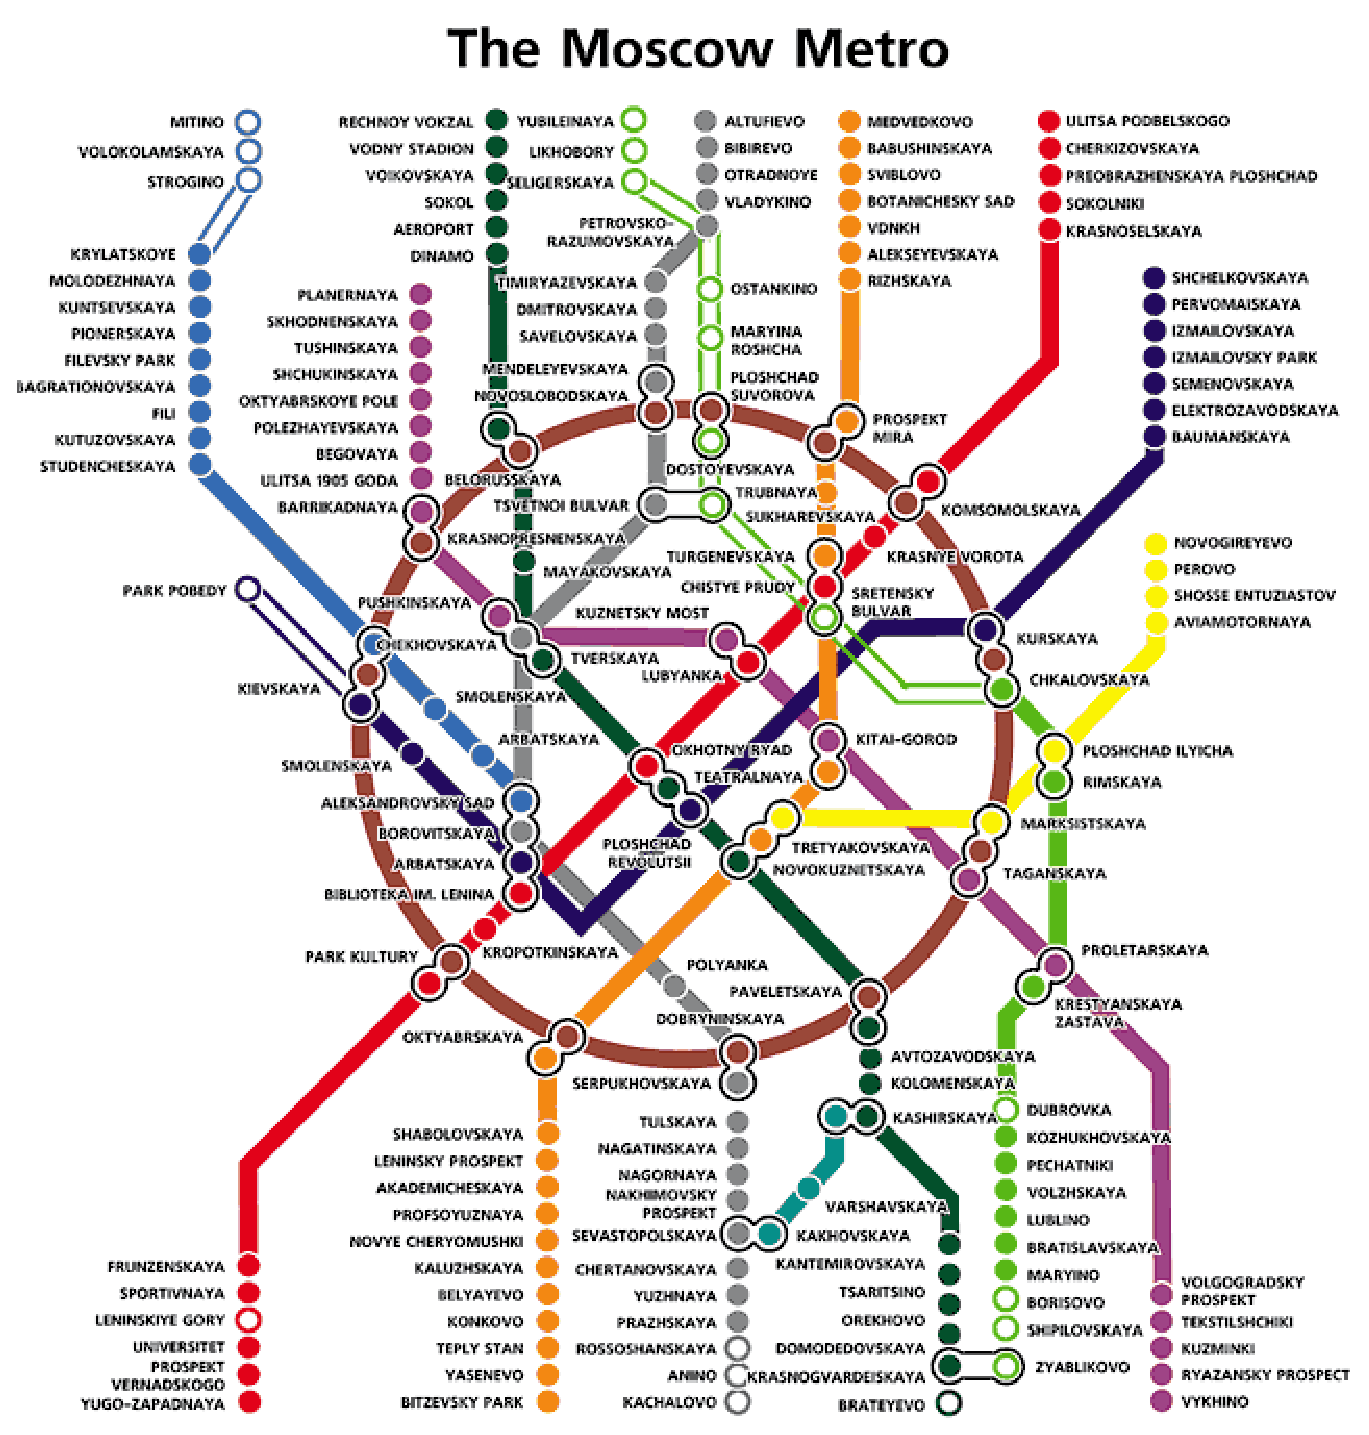
\includegraphics[width=8cm]{Pics/subway_map}
\end{center}
\caption[Example topological map.]{An example of a topological map, the Moscow subway map.}
\label{fig:subway}
\end{figure}

With a topological map, the robot is restricted to the routes along
the edges of the map. The robot cannot take shortcuts even if they are
physically possible. 

%TODO: cite topological papers

Metric maps are generally more detailed and hence useful. 
The robot pose and the map features are defined in a single
reference frame. Metric maps can have landmarks (unique or identical),
or they can represent the environment as an occupancy grid. Each cell
of an occupancy grid map is assigned a probability value of being
``occupied by an obstacle''. A hybrid metric map, that combines
landmarks and occupancy grids has also been proposed in
\cite{guivant04}.  

%%% The most common approach to Simultaneous Localisation and Mapping
%%% (SLAM) is based on Extended Kalman Filter
%%% \cite{ekf_slam,dissanayake01}. A more recent development is FastSLAM
%%% \cite{fastslam,nieto2003} and a continuation of this work
%%% FastSLAM 2.0 \cite{fastslam2}.


\section{Localisation} 
\label{sec:Localisation}

%What is localisation
%Typically the robot
%uses a collection of sensors to collect observations of the 
%Why does the robot need to localise
%Topological vs Metric
%Subclasses of the localisation problem

Robot localisation, estimating the pose of a robot, is one of the
fundamental problems in the field of mobile robotics. It is considered
one of the prerequisites for providing autonomous capabilities for a
mobile robot \cite{Cox91}.  The localisation algorithm can face three
possible problems

\begin{itemize}
\item {\bf Position tracking}\\
      The robot's initial pose is known with relatively high
      certainty. The robot keeps track of its pose as it moves through a
      familiar environment.

\item {\bf Global Localisation}\\ 
      The initial pose of the robot is unknown, or is given by a
      probability distribution $p(\x{0}{}{})$ with high variance. As
      the robot moves through the environment and collects
      observations, it determines its pose.

\item {\bf Kidnapped robot}\\ 
The robot is moving through the environment and is reasonably certain
about its pose. Suddenly it gets moved by an external force (think of
a robotic vacuum cleaner) to some other place within a known map. The
robot should be able to detect that its estimate of the pose is no
longer correct and re-localise.
\end{itemize}

Much research has previously concentrated on position tracking - in
fact many existing algorithms address only the first problem (see
review in \cite{Borenstein96}). Global localisation and the Kidnapped
robot problems have been addressed using multi-hypothesis Kalman
filters \cite{JensfeltKristensen01,Cox94}, Markov localisation
\cite{Fox99}, and Monte Carlo methods \cite{Thrun00j}.


\subsection{Problem Definition}

The problem of localisation can be thought of as a problem of
estimating the probability density distribution of robot pose
conditioned on the observation and control data.  This posterior is
typically called {\it Belief} and is denoted
\begin{equation}
  Bel(\x{k}{}{}) = p(\x{k}{}{} | \Uall{k-1}{}, \Zall{k}{}),
\label{eqn:localise_belief}
\end{equation}
where \Uall{k-1}{} is a set of all control inputs up to time $k-1$, and
\Zall{k}{} is a set of all observations up to time $k$. It is usually
desired to approximate the posterior recursively, otherwise one would
run into computation problems very quickly. Making a Markov
assumption that future data is independent of past data given the
robot pose:
\begin{eqnarray}
 p(\z{k} | \Zall{k-1}{}, \Uall{k-1}{})    &=& p(\z{k} | \x{k}{}{}) \\
 p(\x{k}{}{} | \Zall{k-1}{}, \Uall{k-1}{})&=& p(\x{k}{}{} | \x{k-1}{}{}, \U{k-1}{}).
\end{eqnarray}
By applying Bayes' rule, equation~\refEquation{eqn:localise_belief} is
transformed into a recursive formula (see \cite{Thrun00j} for a
derivation)
\begin{equation}
Bel(\x{k}{}{}) = \eta p(\z{k} | \x{k}{}{}) \int 
                     p(\x{k}{}{} | \x{k-1}{}{}, \U{k-1}{}) 
                     Bel(\x{k-1}{}{}) d \x{k-1}{}{},
\label{eqn:localise_recursion}
\end{equation}
where $\eta$ is a normalisation constant. To implement the recursive
rule in \refEquation{eqn:localise_recursion} one needs to know the
distributions $p(\z{k} | \x{k}{}{})$ and $p(\x{k}{}{} | \x{k-1}{}{},
\U{k-1}{})$. These distributions are generally referred to as {\it
observation} (or sometimes {\it perception}) and {\it motion} models,
respectively. 

The motion model reflects the uncertainty in robot dynamics, so it is
generally independent of time $k$. The observation model is a function
of robot sensors and of the environment. If sensor characteristics do
not change with time and if features in the map are static (a common
assumption), the same observation model can be used for every time
step.

\subsection{Common Approaches to Metric Localisation}

%EKF
Several approaches to localisation have been proposed. One family of
algorithms use the Extended Kalman Filter\cite{Jensfelt99}. Approaches
based on the EKF linearise motion and observation models and
approximate the posterior distribution with a Gaussian. While being
computationally efficient, EKF based approaches have some
limitations. They are not capable of global localisation, hence the
initial pose of the robot should be known with relatively high
confidence. An EKF is only capable of representing a uni-modal
posterior distribution, meaning that in an ambiguous situation only
one of the position hypotheses can be considered. This can lead to
localisation failure if the wrong choice is made.

A mixture of Gaussians model can be used to allow for multiple
hypotheses \cite{JensfeltKristensen01,Cox94}, but the problems arising
from linearisation are still present in these approaches.

%Markov
Markov localisation uses a grid to model the posterior distribution
\cite{Fox99}. This approach is capable of global localisation, and can
deal with the kidnapped robot problem as well. Fox \etal\ \cite{fb99}
have shown that Markov localisation works well, even in highly crowded
environments. The main advantage of this approach is the ability to
model any complex distribution. This makes the algorithm more robust
and allows for global localisation. Drawbacks include finite grid
size, computational demands and the need for a complex implementation
to optimise the observation update and increase resolution ``on the
fly''.

%PF
Particle filter localisation (also known as Monte Carlo localisation)
algorithms model the posterior distributions as a set of particles
\cite{Thrun00j, JensfeltAustinWijk00b}. A particle filter is capable of
approximating any probability distribution, including multi-modal
distributions. It can perform global localisation and can be used to
solve the kidnapped robot problem. Unlike grid-based algorithms,
particle filters have a floating point resolution for robot pose, and so
can give a more accurate pose estimate. Although it is computationally
more demanding than EKF approaches, the increased robustness of this
algorithm makes it worth the additional computational resources. The
computational complexity of the particle filtering algorithm is $O(N)$
in the number of particles used to represent the robot pose. Increasing
the number of particles will result in greater accuracy and
robustness. It is therefore straightforward to trade off the
computational resources against performance.

\section{Simultaneous Localisation and Mapping}
\label{sec:SLAM}

\subsection{SLAM Problem}

This section introduces the problem of Simultaneous Localisation and
Mapping \cite{smith1990eus,thrun2003rms}. 

A robot starts at time 0 at location \x{0}{}{}, executes a series of
motion commands $\Uall{k}{} = [\U{0},\U{1}...\U{k}]$ and collects a
set of observations at every step
$\Zall{k}{}=[\z{0},\z{1}...\z{k}]$. In practice observation and motion
commands are not synchronised, however this can be easily accommodated
in the implementation. It is therefore commonly assumed that
observation and motion happen at the same discrete time interval.
Control and perception of the robot are subject to noise.

SLAM seeks to find the true path of the robot up to time $k$,
$\Xall{k}{}{} = [\x{0}{}{}, \x{1}{}{}, ... \x{k}{}{}]$, and the true
model of the environment, $\map{k}{}{}$. Since there is an inherent
uncertainty in the robot's observation and motion, one generally
cannot give an exact description of the robot's path and a map of the
environment. However, it is possible to construct a probabilistic
model that assigns a likelihood to every path-map combination given
all the available observations, control inputs and the initial pose of
the robot:

\begin{equation}
 p(\Xall{k}{}{}, \map{k}{}{} | \Zall{k}{}, \Uall{k}{}, \x{0}{}{}).
\label{eqn:map}
\end{equation}

Assuming that odometry errors are independent of the observation
errors and of the environment model, one can separate the model into
an observation and motion parts and define:

\begin{enumerate}

\item The model of the robot's motion $P(\x{k}{}{} | \Uall{k}{})$. \\
If one makes a further assumption that past odometry errors have no
effect on future errors, one can represent robot motion as a Markov
process, with probability distribution 
\begin{equation}
 P(\x{k}{}{} | \Uall{k}{}) \equiv p(\x{k}{}{}| \x{k-1}{}{}, \U{k}).
\end{equation}


\item The model of the robot's perception
$p(\z{k}| \x{k}{}{},\map{k}{}{}, \Zall{k}{})$.\\
Here again an assumption is made that errors in the measurements are
independent of past errors, hence

\begin{equation}
p(\z{k}| \x{k}{}{},\map{k}{}{}, \Zall{k}{}) \equiv 
  p(\z{k}| \x{k}{}{},\map{k}{}{}).
\end{equation}

\end{enumerate}

Equipped with the knowledge of these distributions one can in
principle compute the exact posterior by considering every possible
path, map and data association decision combination. In practice,
however, computing such a distribution exactly is not possible due to
the high dimensionality of the system. Reasonably good approximations
can, however be obtained, and can be computed incrementally in
real-time.

The two most common approaches to solving the SLAM problem are the EKF
based algorithm \cite{ekf_slam} and a particle filter algorithm called
``FastSLAM'' \cite{fastslam}.

\subsection{Kalman Filter Approach}
The Extended Kalman Filter approach treats the SLAM problem as a state
estimation problem in which the state consists of the robot pose and
locations of all landmarks. Usually the number of features is not
known in advance, so most implementations have some provision for
adding new elements to the map as new observations are obtained. EKF
SLAM requires linearisation of the robot's motion and perception
models, so that the estimation error can be modelled by a Gaussian
distribution.  The computation complexity of the algorithm is
$O(K^2)$, where $K$ is the number of features in the map
\cite{ekf_slam}.

Considerable research has addressed the computational performance of
the EKF approach to SLAM \cite{williams:acra2001, williams2001esa,
  knight2001tct, guivant01, tim_bailey, uhlmann97nondivergent,
  tardos02:_mappin_local_indoor_envir_using_sonar_data}.  It is
possible to exploit the fact that only a small subset of the whole map
is observed at any given time to reduce the computational burden.
Compressed EKF \cite{williams:acra2001} is an optimal approach that
reduces the computational cost of measurement update to $O(K_a^2)$,
where $K_a$ is a number of features in the local region of the global
map.  This approach still requires a costly $O(K^2)$ global
registration stage when robot changes from one local region to the
next. A sub-optimal version of the same algorithm bounds the cost of the
global registration stage.


The most important limitation of the EKF approach is the inability to
model multiple data association decisions. Every observation has to be
classified as noise, a new feature or an observation of an existing
feature.  It is possible to postpone the final decision by running
multiple Kalman filters in parallel. Alternatively, one can try to
improve the quality of data association decisions. Batch data
association techniques like
\cite{neira01:_data_assoc_stoch_mappin_using,
tardos02:_mappin_local_indoor_envir_using_sonar_data} can reduce the
ambiguity of data association, but it is impossible to eliminate this
problem completely. It is impossible to undo incorrect data association
in EKF, as a result EKF is quite sensitive to data association
errors. Detecting large cycles is a very difficult problem for EKF SLAM,
due to the inability to deal with ambiguous data association.


\subsection{Particle Filter Approach}
FastSLAM uses particles to approximate the posterior distribution
\cite{fastslam}. Every particle maintains its own path, data
association decisions and the resulting map. The map is a collection
of independent landmarks. Particle locations are estimated using a
Kalman filters for every landmark. FastSLAM requires linearisation of
the perception model, but it samples directly from the motion model.
As a result, no change to the motion model is required. FastSLAM can
be implemented in $O(M\log K)$, where $M$ is the number of particles
and $K$ is the number of landmarks.

Given enough particles, FastSLAM produces a reasonable estimate of the
posterior distribution. Unfortunately it is not clear how many particles
are needed for a particular problem. A modified version of the FastSLAM
algorithm \cite{fastslam2} uses an alternative sampling technique to
generate particles where they are needed most, therefore reducing the
number of particles needed. The authors \cite{fastslam2}, demonstrate
that in some cases even one particle is enough.

The main advantage of FastSLAM is its ability to handle multiple data
association decisions \cite{Montemerlo2003}, which makes it a more
robust algorithm. From the implementation perspective, FastSLAM is
trivial to parallelise since computation per particle is independent
of other particles. This allows implementations to exploit the recent
trend towards larger numbers of processors, rather than faster
processors, in emerging computational hardware.

\subsection{Effect of Ambiguous Data Association on Posterior
  Distribution}
\label{sec:AmbiguousDA}

One of the advantages of the EKF - representing a posterior
distribution as a Gaussian, is also a weakness. Linearisation allows
for an efficient implementation and provides a sound mathematical
background for the algorithm. However, posterior distributions arising
in SLAM can be distinctly non-Gaussian depending on the environment,
robot dynamics and sensor characteristics.

One of the factors affecting the true posterior distribution is the
quality of data association decisions. In the case of perfect data
association, the posterior distribution tends to have a single peak
and can be approximated with a Gaussian quite well. When data
association is unreliable, multiple plausible hypothesis for data
association arise. These multiple hypothesis produce a multi-modal
posterior distribution.

\begin{figure}
\begin{center}
\subfigure[Experiment setup]{
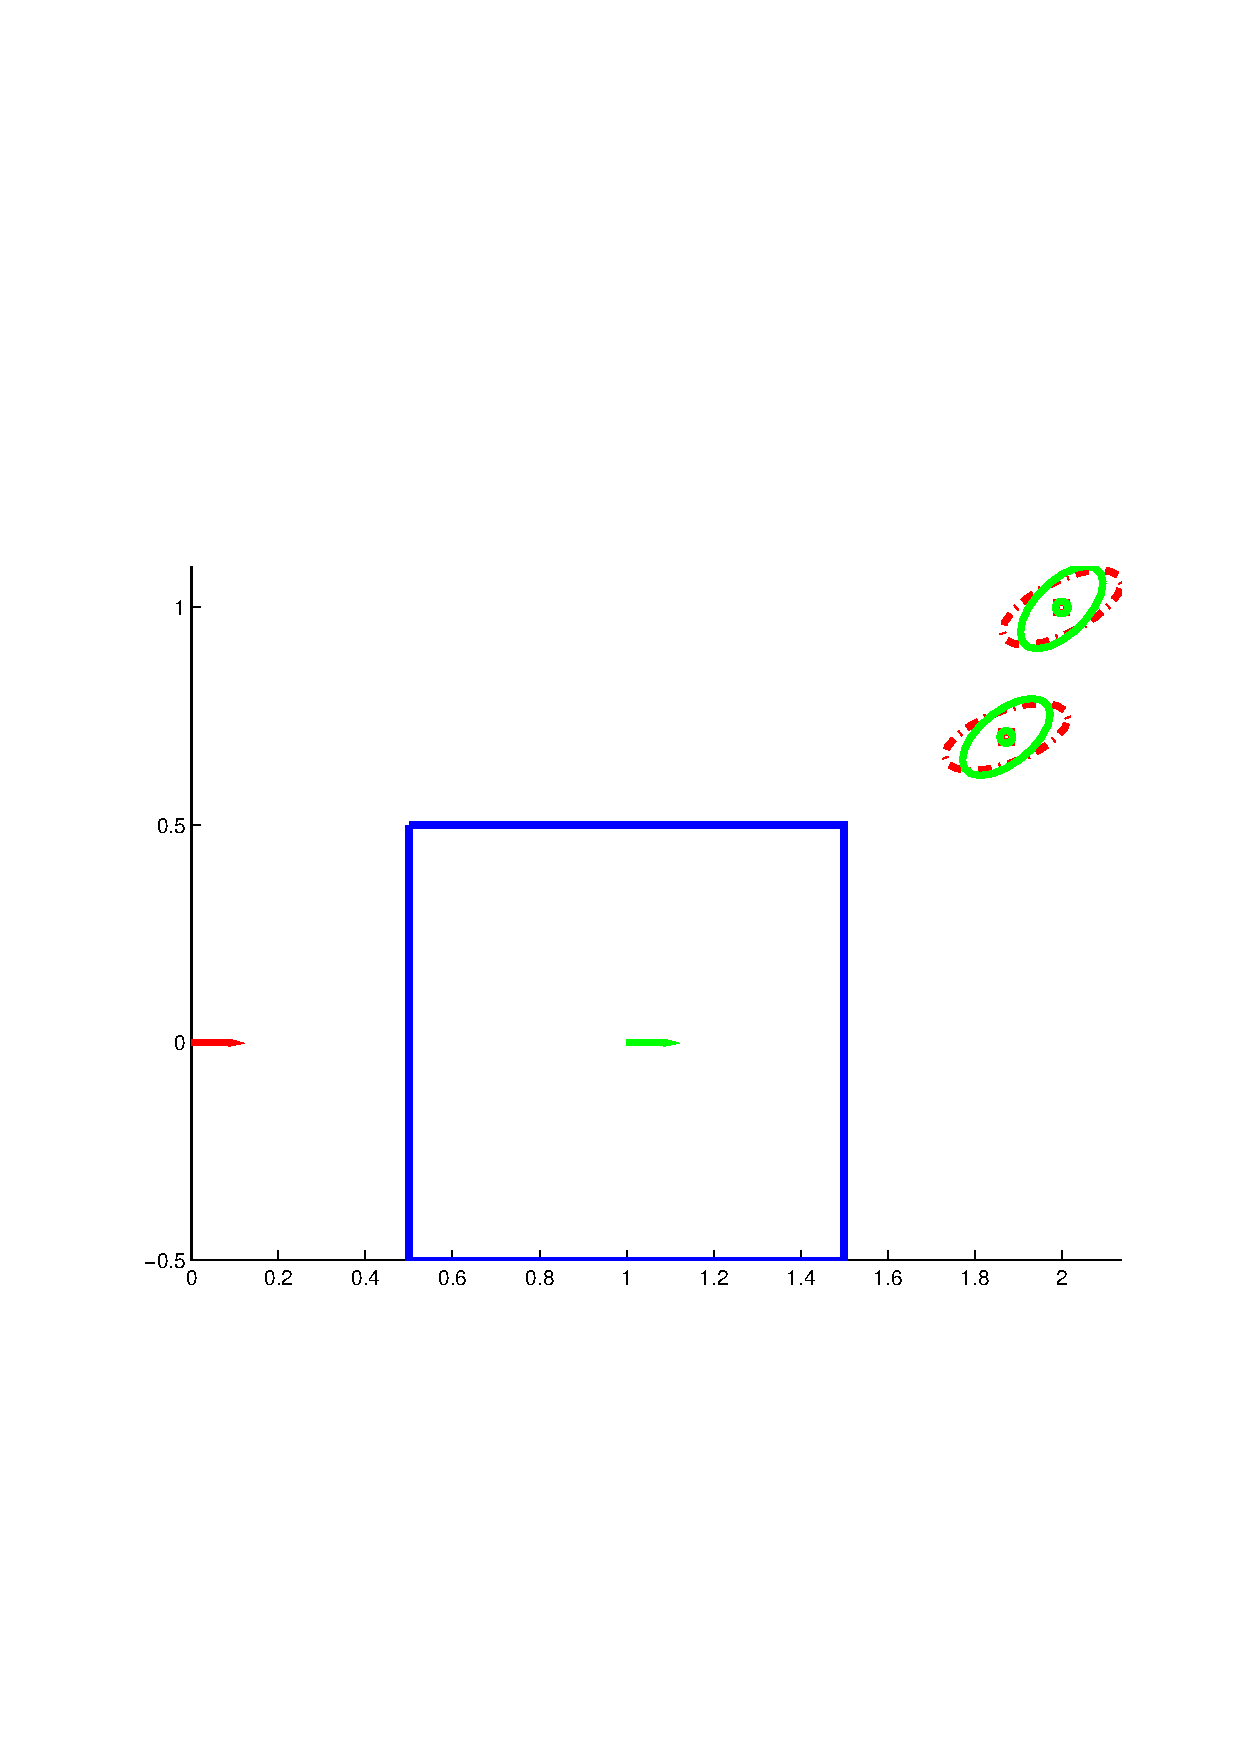
\includegraphics[width=6cm]{Pics/post_example}
\label{fig:post_example}
}
\subfigure[$p({\bf x} | {\bf u})$]{
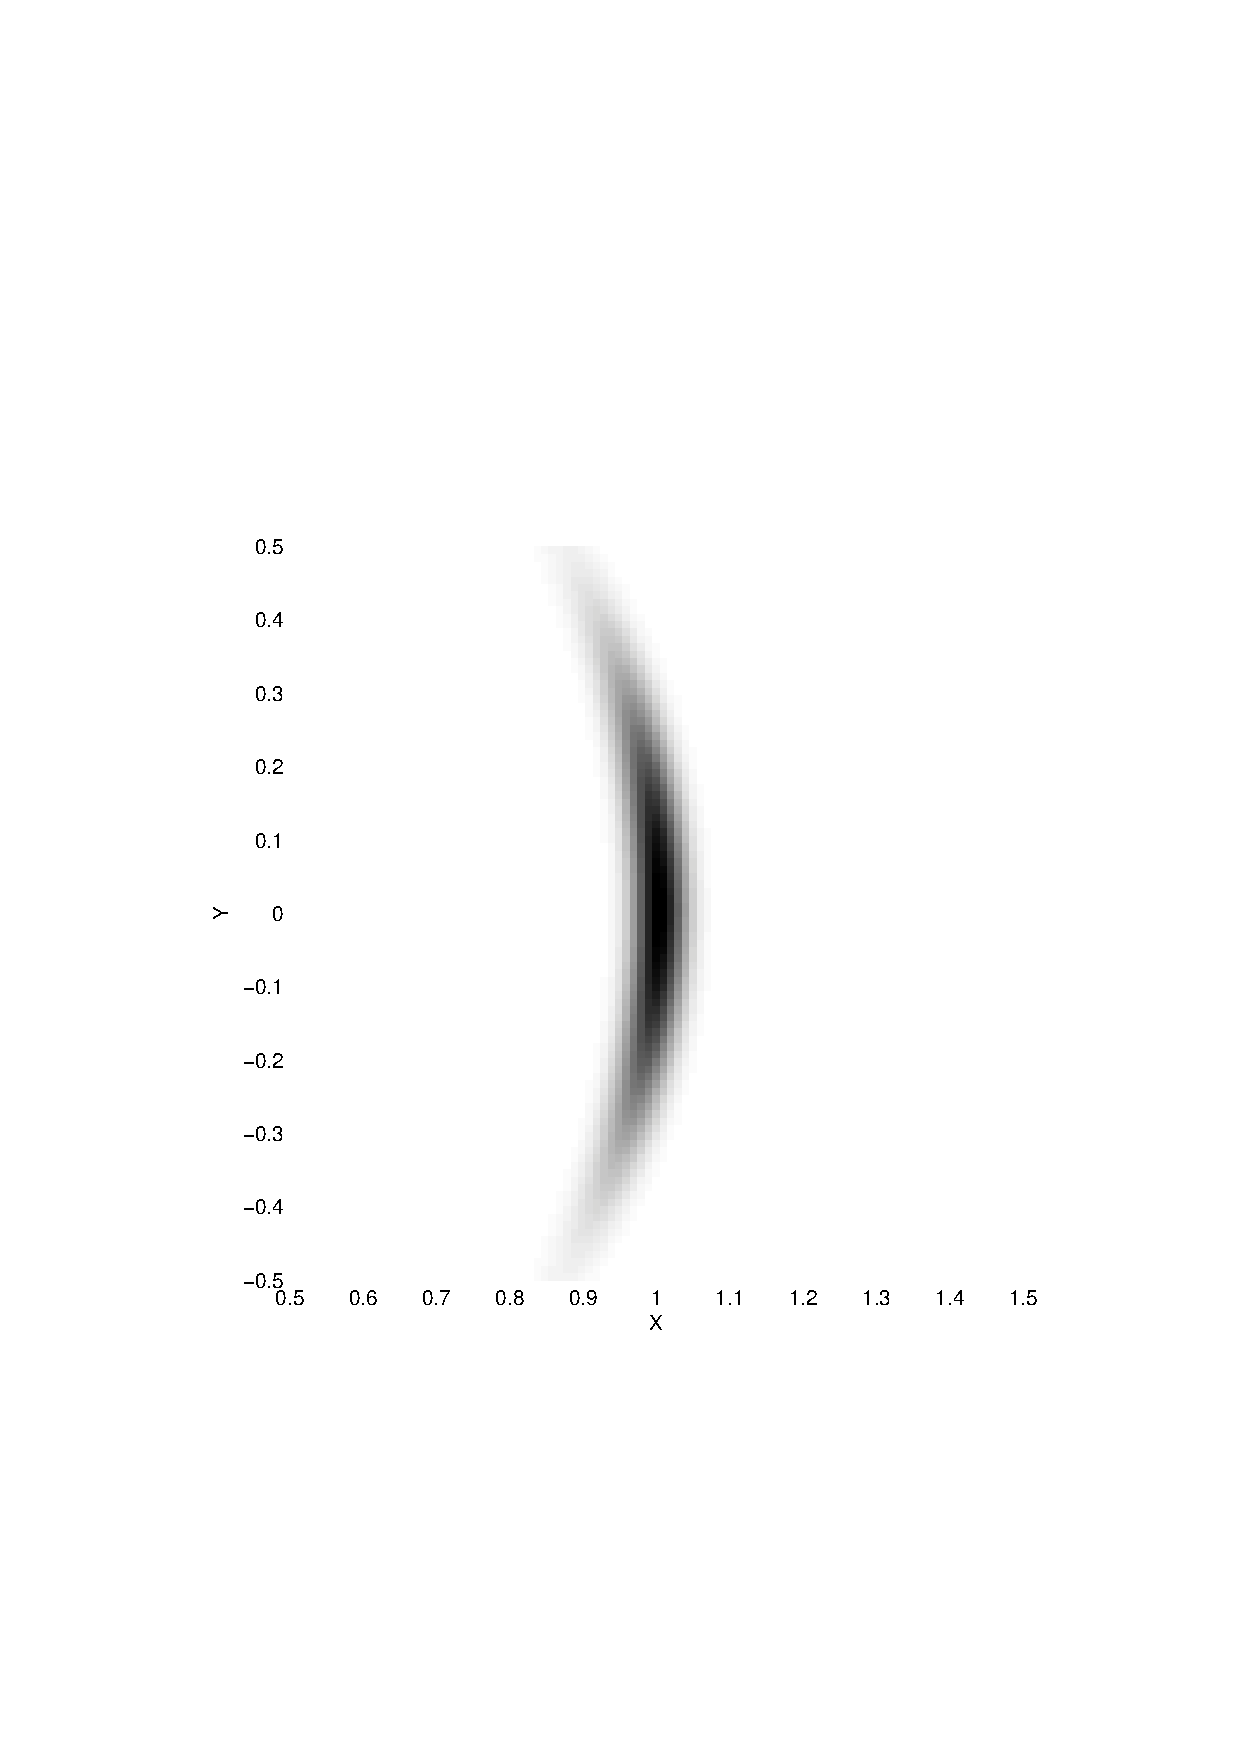
\includegraphics[width=6cm]{Pics/post_odo}
\label{fig:post_odo}
}\\
\subfigure[Known data association: $p({\bf x} | {\bf z})$ ]{
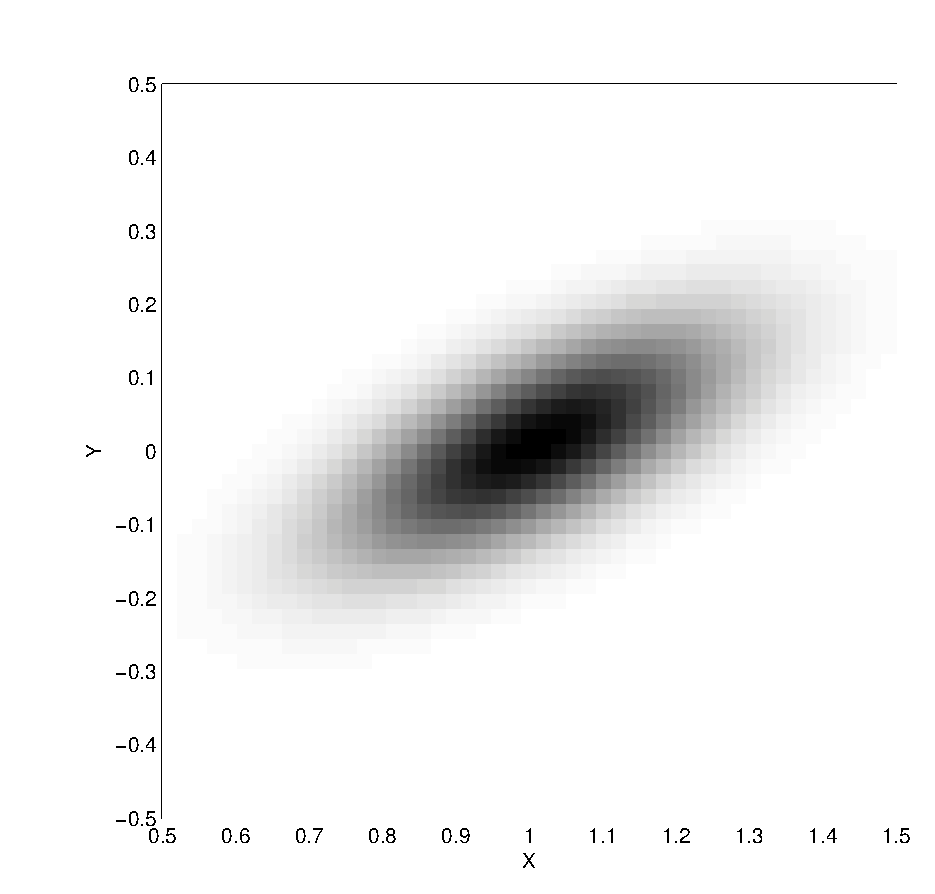
\includegraphics[width=6cm]{Pics/post_obs}
\label{fig:post_obs}
}\quad\space
\subfigure[Known data association: $p({\bf x} | {\bf u},{\bf z})$]{
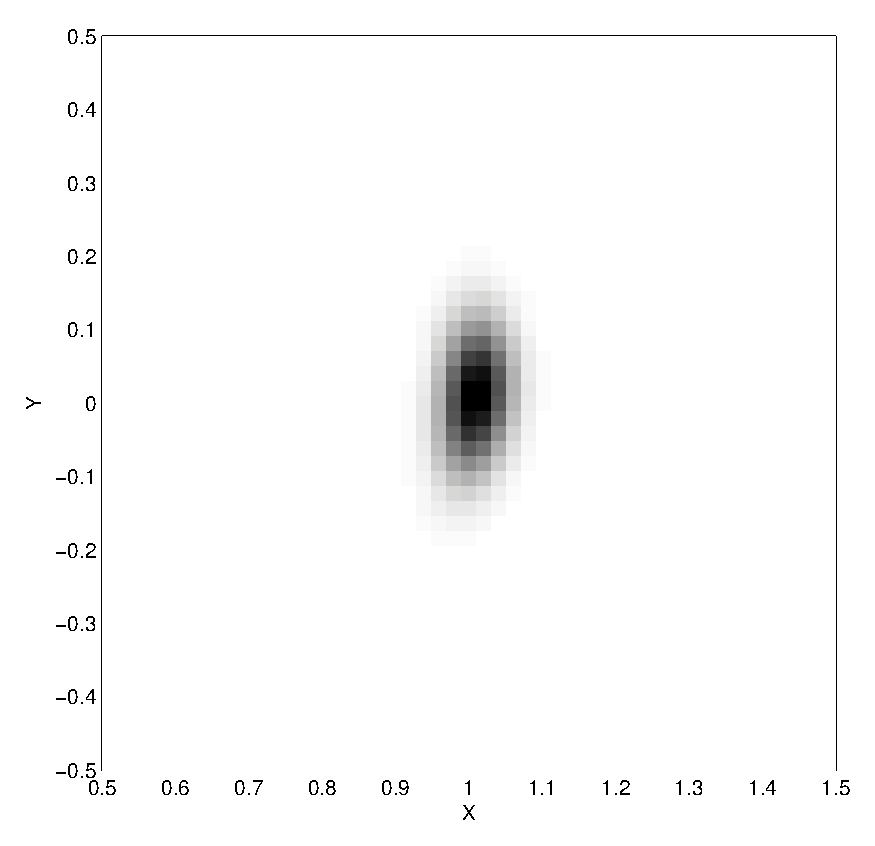
\includegraphics[width=6cm]{Pics/post_obsodo}
\label{fig:post_obsodo}
}\\
\subfigure[Ambiguous data association: $p({\bf x} | {\bf z})$ ]{
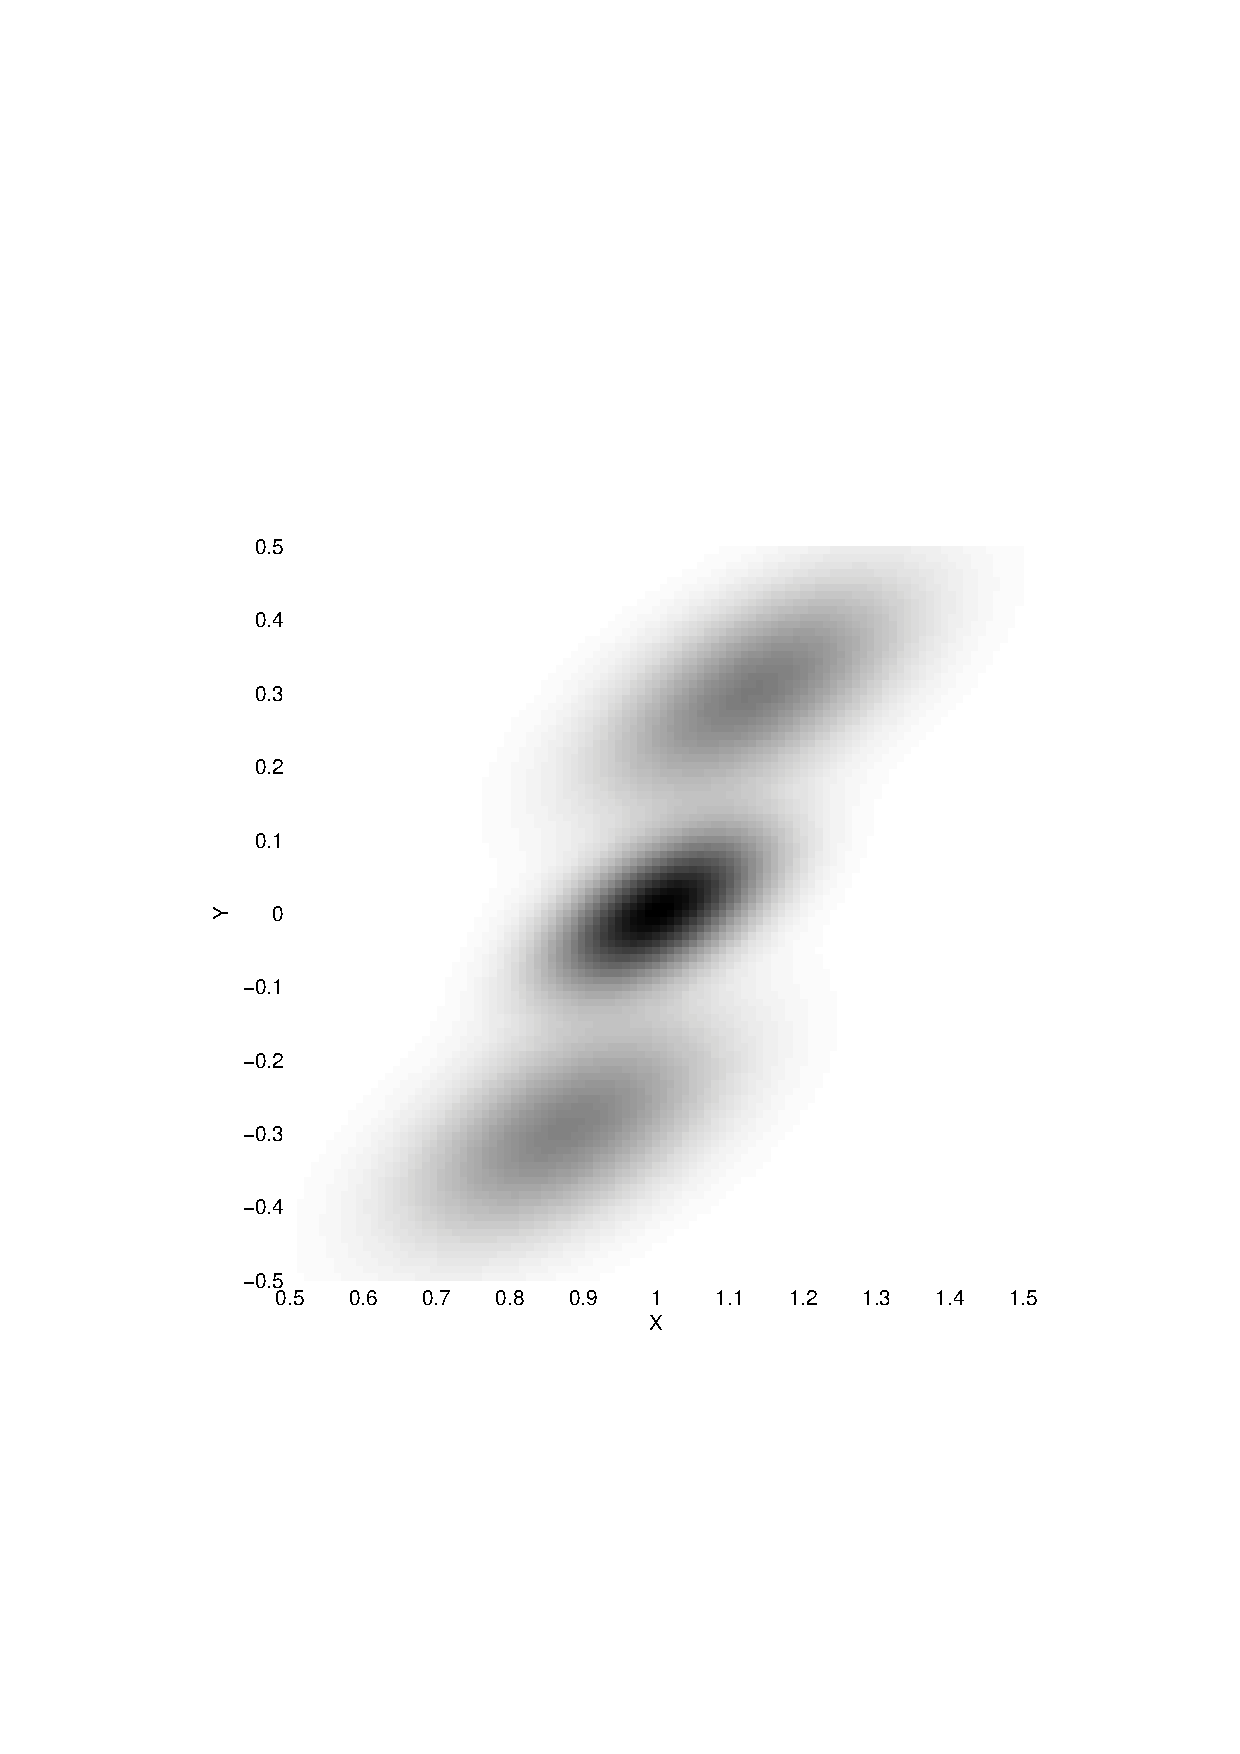
\includegraphics[width=6cm]{Pics/post_obs_}
\label{fig:post_obs_}
}\quad\space
\subfigure[Ambiguous data association: $p({\bf x} | {\bf u},{\bf z})$]{
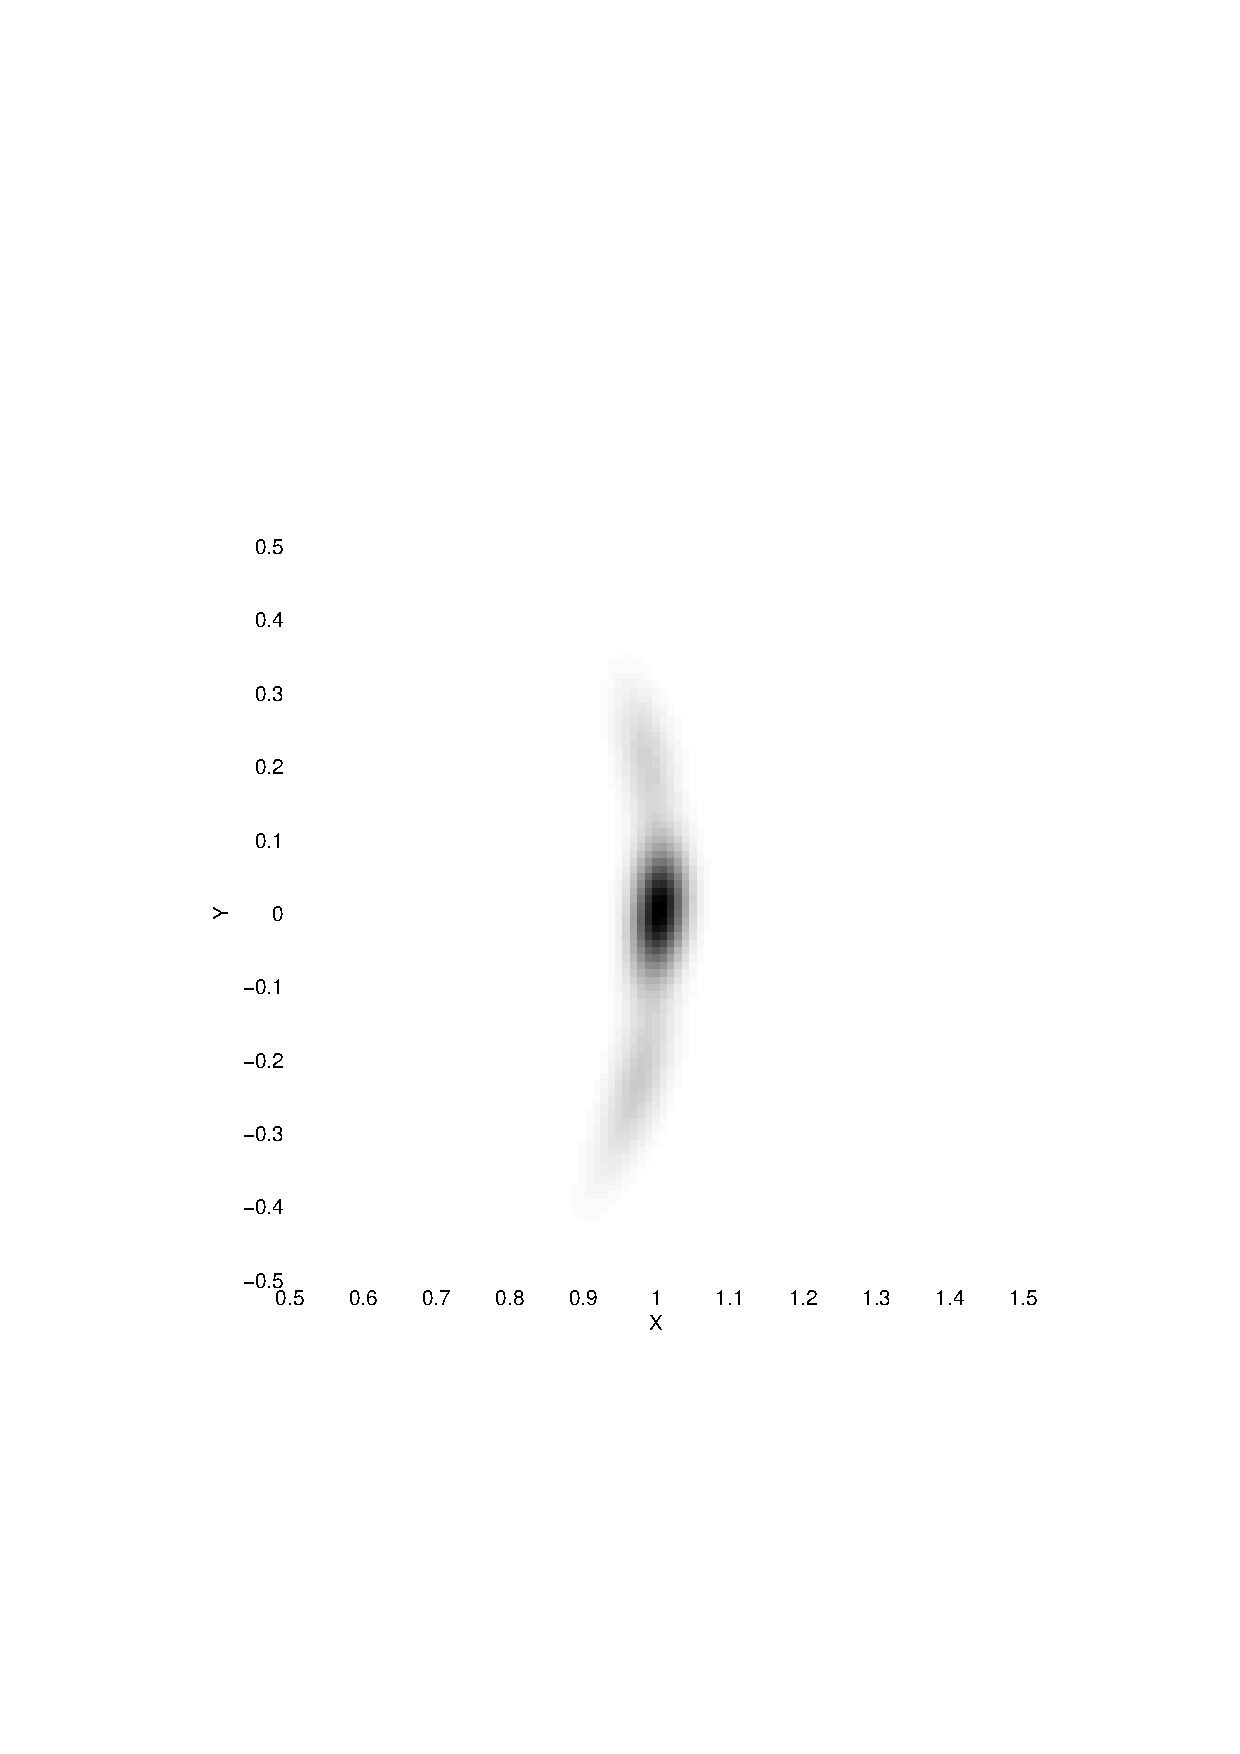
\includegraphics[width=6cm]{Pics/post_obsodo_}
\label{fig:post_obsodo_}
}
\end{center}
\caption[Robot pose uncertainty, example]{In \ref{fig:post_example} a
  robot makes an observation at point (0,0), then moves 1 meter
  forward and makes another observation. The square shows the region
  for which pose uncertainty is computed. The resulting uncertainty
  in robot pose just before the second measurement is shown in
  \ref{fig:post_odo}. Two scenarios are considered: known and
  ambiguous data association (rows two and three respectively).  The
  uncertainty due to the measurement is shown in \ref{fig:post_obs}
  and \ref{fig:post_obs_}. The robots pose uncertainty after
  incorporating the measurement is presented in \ref{fig:post_obsodo}
  and \ref{fig:post_obsodo_}.}\label{fig:post_all}
\end{figure}

To illustrate this point, consider a simple mapping example: the world
consists of two point landmarks and a robot living on a
two-dimensional plane, as shown in \refFigure{fig:post_all}. Robot
pose is defined by its location on the plane only, ignoring the
orientation of the robot (one can assume that the robot has an
extremely accurate compass). The robot is equipped with a sensor that
reports landmark location relative to the robot pose. The error of the
sensor is zero-mean Gaussian.

The robot makes an observation at point (0,0), then moves one meter
forward and makes another observation,
see \refFigure{fig:post_example}. The robot dynamics are controlled by
the following equation:
$$
  \Vector{x_k\\y_k} = \Vector{ x_{k-1} + r_k cos(\Theta_k)\\
                               y_{k-1} + r_k sin(\Theta_k) },
$$
here control inputs at time $k$ are $r_k$ and $\Theta_k$ for distance
and direction of travel, respectively. Gaussian noise in actuation
produces a banana-shaped distribution over the robot pose, shown in
\refFigure{fig:post_odo}.

Consider first the scenario when data association is perfect. After
execution of the motion command the robot observes the landmarks once
more. Since the observations were not certain for both first and
second observation, the pose estimate that can be derived from the
measurements has a significant uncertainty. This is illustrated in
\refFigure{fig:post_obs}. The posterior distribution is non-Gaussian
in this case as well, although the difference is not as apparent as in
the motion example. The posterior distribution of the robot pose given
observations and control input is shown in
\refFigure{fig:post_obsodo}, while it is not strictly Gaussian, it can
be argued that it can be approximated by a Gaussian reasonably well.

In the case when data association is ambiguous, the posterior
distribution is slightly more complicated. Lets assume the robot has
three equally likely data association hypotheses. 

\begin{itemize}
\item Observations 1 and 2 map to landmarks {\bf a},{\bf b}
\item Observation 1 maps to landmark {\bf b}, observation 2 is spurious
\item Observation 2 maps to landmark {\bf a}, observation 1 is spurious
\end{itemize}

Each of these hypotheses by itself produces an almost Gaussian
posterior distribution, but when combined the result is a multi-modal
distribution shown in \refFigure{fig:post_obs_}. The posterior
distribution of the robot pose given observations and control input is
then as shown in \refFigure{fig:post_obsodo_}. Clearly this
distribution differs significantly from a Gaussian.

The presented example shows that non-Gaussian distributions in robot
posterior can arise as a result of an ambiguous data
association. Approaches to SLAM that can deal with such distributions
therefore might have an advantage in such situations.


\section{Loop Closing}
\label{sec:back_loop}
%Problem definition
  % Detect
  % Correct

The problem of loop closing arises when mapping a large cyclic
environment. When the robot returns to a previously mapped region via
a large loop, rather than by back-tracing its own steps, it needs to
recognise the place as previously mapped. Failure to do so will result
in inconsistent map.  As the robot moves through an unexplored
environment while building the map, it becomes more and more uncertain
about its pose relative to the regions it mapped in the past.
Increased uncertainty in robot pose makes it more difficult to
detect a place the robot has already mapped.

%The increase in the uncertainty makes it hard for the robot to detect when it comes
%back to the region it has mapped already. 
%Failure to detect revisiting results in an inconsistent map.

In order to build a consistent map, the robot needs to be able to
detect the places it has visited to before and correct its estimate of
the path along the loop. The problem of mapping large cyclic
environments has been addressed by several researchers.


%what is there now
  %Lu Milios (scan matching + optimisation)
  %Gutman   (scan matching + confirm + handles high uncertainty)
  %Thrun's  (EM)
  %Fergusson (EKF mines)
  %Atlas


Lu and Milios \cite{lu97:_global} propose an algorithm they call
``consistent pose estimation''. The algorithm uses laser scan matching
and linearised global optimisation over scan poses to build a scan map
of the environment in a single global frame. The approach builds a
network of robot poses at which a laser scan has been taken. The poses
are connected by ``weak'' and ``strong'' links. The links represent
the spatial relations between poses. Weak links are derived from
odometry and strong links are derived from the scan matches. The
algorithm then finds a global configuration of the poses of the places
by minimising a cost function. If one thinks of links as springs, the
algorithm finds the configuration that reduces the sum of forces
exerted by the springs. Spatial relations are modelled by Gaussians,
and the cost function is the sum of the Mahalanobis distances.

The method by Lu and Milios is very sensitive to the initial estimate
of the robot pose just before loop closing. Since the pose estimate is
derived from local scan matching and odometry, it can, in principle,
have unbounded error. If the initial estimate is too far from the true
robot pose, the algorithm tends to converge to spurious local minima.
The method also has high computational complexity, $O(N^3)$ in the number of poses.

Konolige and Gutman
\cite{konolige99:_increm_mappin_large_cyclic_envir} provide a method
based on the ideas of Lu and Milios, but try to address these
problems. Instead of using single laser scan to find relations between
places they use a map correlation technique \cite{konolige99}. This
makes the system more robust to false correspondences. After detecting
loop closing, the algorithm runs consistent pose estimation. 

An interesting scan matching based mapping technique has been
developed by by Ferguson \etal\ \cite{fergusson2003}. In this
approach loop closing can be undone if the observations further down
the track do not support it.

Thrun \etal \cite{slam_thrun98b,Thrun98a,thrun98:_probab} suggest an
approach that uses an Expectation Maximisation (EM) algorithm to
construct maps of cyclic environments. The algorithm is given a
relatively small set of observations of sparsely positioned non-unique
landmarks and the set of all control inputs. In the expectation step the
algorithm computes the most likely robot path given the map and the
data. In the maximisation step the most likely map is computed given
the robots path from the E-step. The Expectation and Maximisation
steps are repeated until the map converges to the maximum likelihood
solution. This algorithm cannot be implemented in real-time because
it needs to have access to all of the future and past data to
determine the robot pose at any given time. %% check maximum likelihood

All of the methods presented so far build a map of the whole
environment in a single global reference frame. Recently, Bosse \etal\
\cite{bosse03atlas} suggest a mapping approach, \Atlas, that does not
require a global reference frame. The map structure used in this
approach is a hybrid topological/metric map.  Each node is a local map
and every link in the topological map represents a spatial
relationship between the two places it connects. 

\Atlas\ uses a combination of map matching and uncertainty projection
to detect when the robot re-enters a previously explored area.
Uncertainty projection computes the relative poses between the two
non-adjacent local maps. If according to this estimate, the two maps
might be overlapping, \Atlas\ tries to find the landmark
correspondences between the two maps. If the two maps match, the new
link is added to the topological map. The pose relation for this link
is computed from the landmark correspondences. In order to decrease
the probability of incorrect data association, \Atlas\ runs several
hypotheses at any given time. If, after closing the loop, the
observations do not match the map well enough, the loop closing
hypothesis will be discarded in favour of the new map hypothesis.


\section{Limitations of Metric Approaches to Mapping}

%Until recently there were two main strategies for map representations
%in robotics: topological and metric. 
%Problems with global mapping.
%Building an accurate metric map is not a trivial matter. 

While there exist several good methods for building metric maps, they
do not scale up to big environments. The main restricting factors are:

\begin{enumerate}
 \item Increase in the computational complexity. The larger the
  environment the longer it takes to execute an update with every new
  measurement.

 \item Increase of the robot pose uncertainty. As you run the
 algorithm for longer, errors tend to accumulate, especially in large
 environments. No matter how accurate your mapping process is,
 there is still going to be some residual uncertainty, and it will
 accumulate as the robot travels longer distance. The effect of such approximation
 errors is especially harmful when cycles are present.

 \item Increasing approximation error in the mapping procedure.

\end{enumerate}

The first point is fairly obvious: more landmarks require more
computation and more memory. Since the environment is considered as a
whole, one needs access to all landmarks to continue mapping. This
problem was tackled by Williams \etal\ using Constrained Local Submap
Filters \cite{williams:acra2001}. Their approach uses local maps for
building the immediate environment around the robot, effectively
forgetting about the rest of the world. The local map is then merged
into the global reference frame. This keeps the computational
requirements relatively constant, irrespective of the environment
size. The underlying mapping algorithm used in this approach is EKF
SLAM.

Increasing uncertainty is another fundamental problem when a map is
built incrementally, i.e. new measurements are added to the existing
map as they arrive. In order to add a measurement the robot needs to
solve a data association problem: is this observation from one of the
features already in the map, is it new or is it noise?  As the robot's
pose uncertainty in the existing map increases, data association
becomes more difficult. An incorrect data association decision becomes
more likely, leading to inconsistent maps. Even in the case when
perfect data association is possible (when unique landmarks are used),
increasing pose uncertainty will cause problems, since pose
uncertainty also means map uncertainty. Even if the robot manages to
re-localise itself, correcting the map can be a problem.

The problem of data association under uncertainty has been addressed
by \cite{neira01:_data_assoc_stoch_mappin_using,
  tardos02:_mappin_local_indoor_envir_using_sonar_data}.  Rather than
finding the mapping of a single observation to a landmark, these
approaches consider a set of observations simultaneously. While such
approaches make data association more robust to sensor pose
uncertainty, they do not completely resolve the problem of {\it
  increasing} uncertainty.


Algorithms that work on all of the data at once, like Expectation
Maximisation \cite{thrun98:_probab}, are not affected by this problem,
but their computational requirements are huge and they cannot operate
in real time, since all of the data has to be processed at once.

In the case of FastSLAM, data association is solved on a per particle
basis. Data association is therefore not affected by the increasing
uncertainty. FastSLAM can also correct the map after loop closing
automatically and in real time, by simply keeping only the ``good''
particles. Nevertheless the increasing uncertainty is still a
problem. In order to perform reliably, FastSLAM will require more and
more particles to accurately represent the increasing robot pose
uncertainty. Like any particle filtering algorithm, FastSLAM is
affected by the particle depletion problem: if there are not enough
particles in the right region, the algorithm will fail to detect a
loop-closing.

EKF SLAM tends to underestimate robot pose uncertainty, and as a
result it might fail to detect loop closing. Correcting the map and
the path, even if the robot does re-localise itself, is also a big
problem for EKF SLAM, and does require substantial computational
resources.

Another important limitation comes from the approximation error. Every
mapping algorithm is trying to compute the map as a joint posterior
distribution of robot poses and a map given all the observations and
control inputs. Since computing such a distribution in its true form
is rather impractical, all existing approaches try to approximate it.
As the environment size increases the effect of approximation becomes
more significant.

%%% EKF SLAM linearises the motion and observation models. FastSLAM
%%% approximates the robot pose by the set of particles, and assumes a
%%% Gaussian observation model. EM based SLAM has to make some assumptions
%%% about the environment and the robot motion. 


\section{Hybrid Approaches to SLAM} 

If one segments the environment into a number of smaller regions, and
maps each region separately (build local maps), one can avoid the
problem of unbounded complexity and also reduce the effects of
approximation errors.

Hybrid topological/metric maps
\cite{fergusson2003,bosse03atlas,Thrun98a} allow for accurate local
positioning by virtue of the metric component, yet are easier to
construct since computational complexity per local map is bounded. It
is also easier to close large cycles since closing a cycle in such a
map is just a matter of adding a link between two places in the
topological structure of the map.

%%% Existing hybrid approaches can be grouped into three broad
%%% categories: mainly metric, mainly topological, and truly hybrid. 
%%% 

Some of the hybrid methods desire to build a global metric map
\cite{Thrun98a, slam_thrun98b}. These approaches use topological
structure as an intermediate step only. The environment is split into
local maps, each local map is explored separately, and all maps are
then merged into a large, global map. Merging can happen incrementally
or as a single post-processing step. Some optimisation steps might be
used to enforce consistency of the global map. The main advantage of
such methods is a more robust loop closing behaviour. This is due to
the fact that loop closing is performed based on map matching.

Other methods build topological maps with independent metric maps for
each node \cite{Cho01,Kuipers00}. Metric maps are built for every node of the
topological map as an after thought. The relationships between nodes
is purely topological. Metric information is only used inside the
local maps.

More recently a tighter coupling of metric and topological
information started to appear in robotic research. A hybrid mapping
approach called \Atlas\ by Bosse \etal\ \cite{bosse03atlas} incorporates
metric information into the topological structure of the map. Every
link in the topological structure stores the spatial relation between
the two nodes (local maps) as a stochastic variable. 

%%% \Atlas\ is described in more detail in the next section.


\subsection{Atlas}

\Atlas\ by Bosse \etal\ \cite{bosse03atlas} is a hybrid
topological/metric approach to SLAM. \Atlas\ models environment as a
set of local maps of bound size. There is no single global reference
frame, only local transformations between adjacent local maps are
maintained. Spatial relationships are approximated by a Gaussian,
derived from the residual robot pose uncertainty of the mapping
process used to build the local maps.

\Atlas\ supports various underlying mapping modules for building local
maps. The two mapping modules presented in \cite{bosse03atlas} were
based on EKF SLAM using line and point features extracted from either
laser or sonar range data.

The main advantage of \Atlas\ is the map structure it uses. Moving
away from the single reference frame allows the mapping of large
environments with huge cycles in real time. Even though there is no
global reference frame, it is still possible to compute the relative
poses of any two local maps with some certainty, hence it is possible
to project the robot pose estimate from one reference frame to any
other, along with the uncertainty.


When closing large cycles, \Atlas\ relies on place recognition
(map matching) and the robot pose estimate to detect a revisiting
event. If the two maps match, and the robot pose derived from the
match is likely, a new link can be added to the topological structure.
In order to avoid false positives, a loop closing hypothesis is first
tested by considering how well the observations match the map.

There are, however, some limitations to this approach. When, for
instance, the robot returns to a previously mapped region it gains new
knowledge about the relative positions of the local maps. The robot
can use this knowledge to update the links in the map. \Atlas\ does
not perform this update because of the computational requirements
involved, although the authors mention that such update can be performed
after the mapping is complete. \Atlas\ uses metrics to test loop
closing hypotheses. These metrics do not necessarily correspond to the
true likelihood, making it difficult to predict the behaviour of the
algorithm in a new environment.

\section{Summary}

The past few decades of mobile robotics research provide powerful
tools for mapping and localisation. Existing algorithms tend to be
limited to relatively small environments. The main limiting factors
are:

\begin{itemize}
\item The computational burden: as size of the environment grows, so do
  the computational requirements of existing algorithms.

\item The data association problem in the face of uncertainty: 
   in large environments the uncertainty of the landmarks far away
  from the origin is high. That makes it difficult to perform correct
  data association.

\end{itemize}

Various optimisation techniques and faster hardware can expand the
capabilities of existing algorithms, but to overcome these limitations
new map representations are required. In particular new ways to model
uncertainty should be explored.

% TODO: my contribution in a paragraph 1-2 sentences.
%TODO: many people worked on EKF, fewer on FastSLAM, no work on PF +
%hybrid map models. Need to explore new data structures, not just keep
%trying to patch up EKF approach.
%We therefore chose to use FastSLAM to perform local mapping tasks.

% Some recent research in
% this area include \cite{bosse03atlas,fergusson2003}.




\nocite{tim_bailey,
bosse03atlas,
fergusson2003,
thrun00,
dissanayake01,
SOG-Slam01,
guivant02:_simul,
guivant02:_solvin,
thrun02:_robot_mappin,
 zunino01:_simul,
 JensfeltKristensen01,
 JensfeltWijkAustin00a,
 JensfeltAustinWijk00b,
 anguelov02,
 hahnel02:_map,
 burgard99:_exper,
 schulz01:_track_multip_movin_objec_mobil_robot,
 castellanos99:_spmap,
 castellanos01:_multis,
 dudek00:_robus_place_recog_local_appear_method,
 konolige99:_increm_mappin_large_cyclic_envir,
 lu97:_global,
 gutmann96:_amos,
 williams:icra2002,
 williams:acra2001,
 Zimmer96,
 slam_kuiper91,
 slam_kuipers88,
 Thrun00j,
 Fox99,
 Cox91,
 Borenstein96,
 kk2002,
 sidenbladh00stochastic,
 Cox94,
 Thrun02h,
 Bennewitz02a,
 Liu01a,
 Dellaert00c,
 nieto2003, 
 konolige99,
 doucetraoblackwellised,
 guivant04,
 newman03,
 vandermerwe00_tr,
 vandermerwe2000,
 wan01unscented,
 unscented,
 Margaret_hybrid_maps,
 kuipers1978,
 KuipersLevitt88,
 Kuipers00,
 Buzan04,
 uhlmann97nondivergent,
 julier97new,
 julier96general,
 julier99scaled,
 doucet98sequential,
 DA_Lazy,
 Kuipers2004,
 kk2004}



% LocalWords:  Sensorimotor Preoperational odometry EKF FastSLAM Kalman Siegel
% LocalWords:  Kuipers Golledge linearise Gaussians linearisation Milios
% LocalWords:  Mahalanobis minima Konolige Gutman Thrun Bosse Submap
